\chapterimage{orange2.jpg}
\chapterspaceabove{6.75cm} 
\chapterspacebelow{7.25cm} 
\chapter{Inequality}
throughout our mathematical journey, equalities are always the very basics of most conclusion, and that is also which we start to learn math for. However, inequalities are not such a know thing as equalities.
Inequalities have many tricky characteristics so that we have to take with care, or things could go wrong. This chapter covers the fundamentals of inequality as a crucial tool for problem-solving in Computer Science.

\section{Inequality basics}
We all know about inequalities, and the first thing to clarify is the relationship between sizes. How to determine the size relationship between certain numbers? Since the basis for comparing "numbers" with each other corresponds to one, it is stipulated on the number line that the points increase from left to right, and therefore the numbers they represent increase in turn. Listed in ascending order, that is:

Let \( a, b \) be two real numbers, and the points on the number line are denoted as \( A, B \) respectively. If \( A \) is to the right of \( B \), we say \( a > b \); if \( A \) is to the left of \( B \), we say \( a < b \); if \( A \) coincides with \( B \), we say \( a = b \).

Thus, for any two real numbers, one and only one of the following three situations must hold:

\[
a > b; \quad a = b; \quad a < b.
\]

The above relationship is also known as the one-dimensional coordinate law.

\[
\begin{aligned}
a > b &\Leftrightarrow a - b > 0 \\
a < b &\Leftrightarrow a - b < 0 \\
a = b &\Leftrightarrow a - b = 0
\end{aligned}
\]

Where the symbol “\( \Leftrightarrow \)” (double arrow), read as "if and only if," means that the truth of two propositions depends on each other. That is to say, if one proposition is true, then the other proposition is also true; conversely, if one proposition is false, then the other proposition is also false.

Based on the derivation of inequalities, in most cases, the above principles are sufficient. The following mathematical laws involve the geometric and algebraic meanings of the sizes of real numbers and the relationship between them. They are the basis for comparing the sizes of two real numbers and for proving inequalities by comparison. Let's review some basic properties of inequalities that are the foundation for our further study.

\begin{itemize}
    \item Symmetry: \( a > b \) if and only if \( b < a \).
    \item Transitivity: If \( a > b \) and \( b > c \), then \( a > c \).
    \item Addition (Subtraction): If \( a > b \), then \( a + c > b + c \).
    \item Multiplication (Division): If \( a > b \) and \( c > 0 \), then \( ac > bc \); if \( a > b \) and \( c < 0 \), then \( ac < bc \).
    \item Exponentiation: If \( a > b \), then \( a^n > b^n \), where \( n \) is a positive integer, and \( n \geq 2 \).
    \item Root Extraction (Power Root): If \( a > b > 0 \), then \( \sqrt[n]{a} > \sqrt[n]{b} \), where \( n \) is a positive integer, and \( n \geq 2 \).
    \item If \( a > b \) and \( c > d \), then \( a + c > b + d \).
    \item If \( a > b > 0 \) and \( c > d > 0 \), then \( ac > bd \).
\end{itemize}
\subsection{Exercises}
\begin{exercise}
    Explain the following statement.
    \begin{enumerate}
        \item If \( a > b \), then \( \frac{a}{c} > \frac{b}{c} \);
        \item If \( ac < bc \), then \( a < b \);
        \item If \( a < b \), then \( \frac{1}{a} > \frac{1}{b} \);
        \item If \( ac^2 > bc^2 \), then \( a > b \);
        \item If \( a > b \), then \( a^n > b^n \).
    \end{enumerate}
\end{exercise}

\textbf{Solution:}

\begin{enumerate}
    \item If \( c > 0 \), multiplying both sides of \( a > b \) by the positive number \( \frac{1}{c} \) preserves the inequality, hence \( \frac{a}{c} > \frac{b}{c} \). If \( c < 0 \), the direction of the inequality would be reversed, which is not given in the condition, hence we assume \( c > 0 \).
    \item Dividing both sides of \( ac < bc \) by \( c \) (assuming \( c \neq 0 \)), we get \( a < b \) because division by a positive number preserves the inequality, and division by a negative number reverses it.
    \item Taking the reciprocal of both sides of \( a < b \) reverses the inequality because \( a \) and \( b \) are on opposite sides of the fraction line, hence \( \frac{1}{a} > \frac{1}{b} \) (assuming \( a, b > 0 \) to avoid division by zero).
    \item Dividing both sides of \( ac^2 > bc^2 \) by \( c^2 \) (assuming \( c \neq 0 \)) preserves the inequality, hence \( a > b \) because \( c^2 \) is positive regardless of whether \( c \) is positive or negative.
    \item Raising both sides of \( a > b \) to a power \( n \) (assuming \( n \) is a positive integer) preserves the inequality because both \( a \) and \( b \) are raised to the same power, hence \( a^n > b^n \).
\end{enumerate}
\begin{exercise}
    Given the inequality \( a > b > 0 \), \( c < d < 0 \), \( f < 0 \), show that:
\[
\frac{f}{a - c} > \frac{f}{b - d}.
\]
\end{exercise}
\begin{proof}
    Since \( a > b > 0 \) and \( c < d < 0 \), then \( a - c > b - d \) because subtracting a smaller negative number is the same as adding a larger positive number. Given that \( f < 0 \), when dividing by a larger positive number, the result is smaller because a negative number divided by a positive number yields a negative result, and the further away the divisor is from zero, the smaller the quotient.

Therefore:
\[
\frac{f}{a - c} > \frac{f}{b - d}.
\]
\end{proof}

\section{Solving Quadratic Inequality}
Recall that, when we solve Quadratic equations, we use discriminant to solve equations, which is also applicable to inequalities.
For a quadratic inequality of the form $ax^2 + bx + c > 0$ or $ax^2 + bx + c < 0$ (where $a > 0$), the solution set can be determined by the discriminant $\Delta = b^2 - 4ac$:
\begin{enumerate}
    \item If $\Delta > 0$, the quadratic equation $ax^2 + bx + c = 0$ has two distinct real roots $x_1$ and $x_2$, and $x_1 < x_2$. The solution set for $y = ax^2 + bx + c$ being greater than zero (when $y = 0$) is for values of $x$ either less than $x_1$ or greater than $x_2$, and the solution set for $ax^2 + bx + c < 0$ is $\{ x \mid x_1 < x < x_2 \}$.
    \item If $\Delta = 0$, then $ax^2 + bx + c = 0$ has one real root, specifically $x_1 = x_2 = -\frac{b}{2a}$. The solution set for $y = ax^2 + bx + c$ being greater than zero is all $x$ except $x \neq -\frac{b}{2a}$, and there is no solution set where $ax^2 + bx + c < 0$.
    \item If $\Delta < 0$, then $ax^2 + bx + c = 0$ has no real roots, and the parabola $y = ax^2 + bx + c$ does not intersect the x-axis. The solution set for $ax^2 + bx + c > 0$ is all real numbers, and there is no solution set where $ax^2 + bx + c < 0$.
\end{enumerate}
\begin{figure}[ht!]
    \centering
    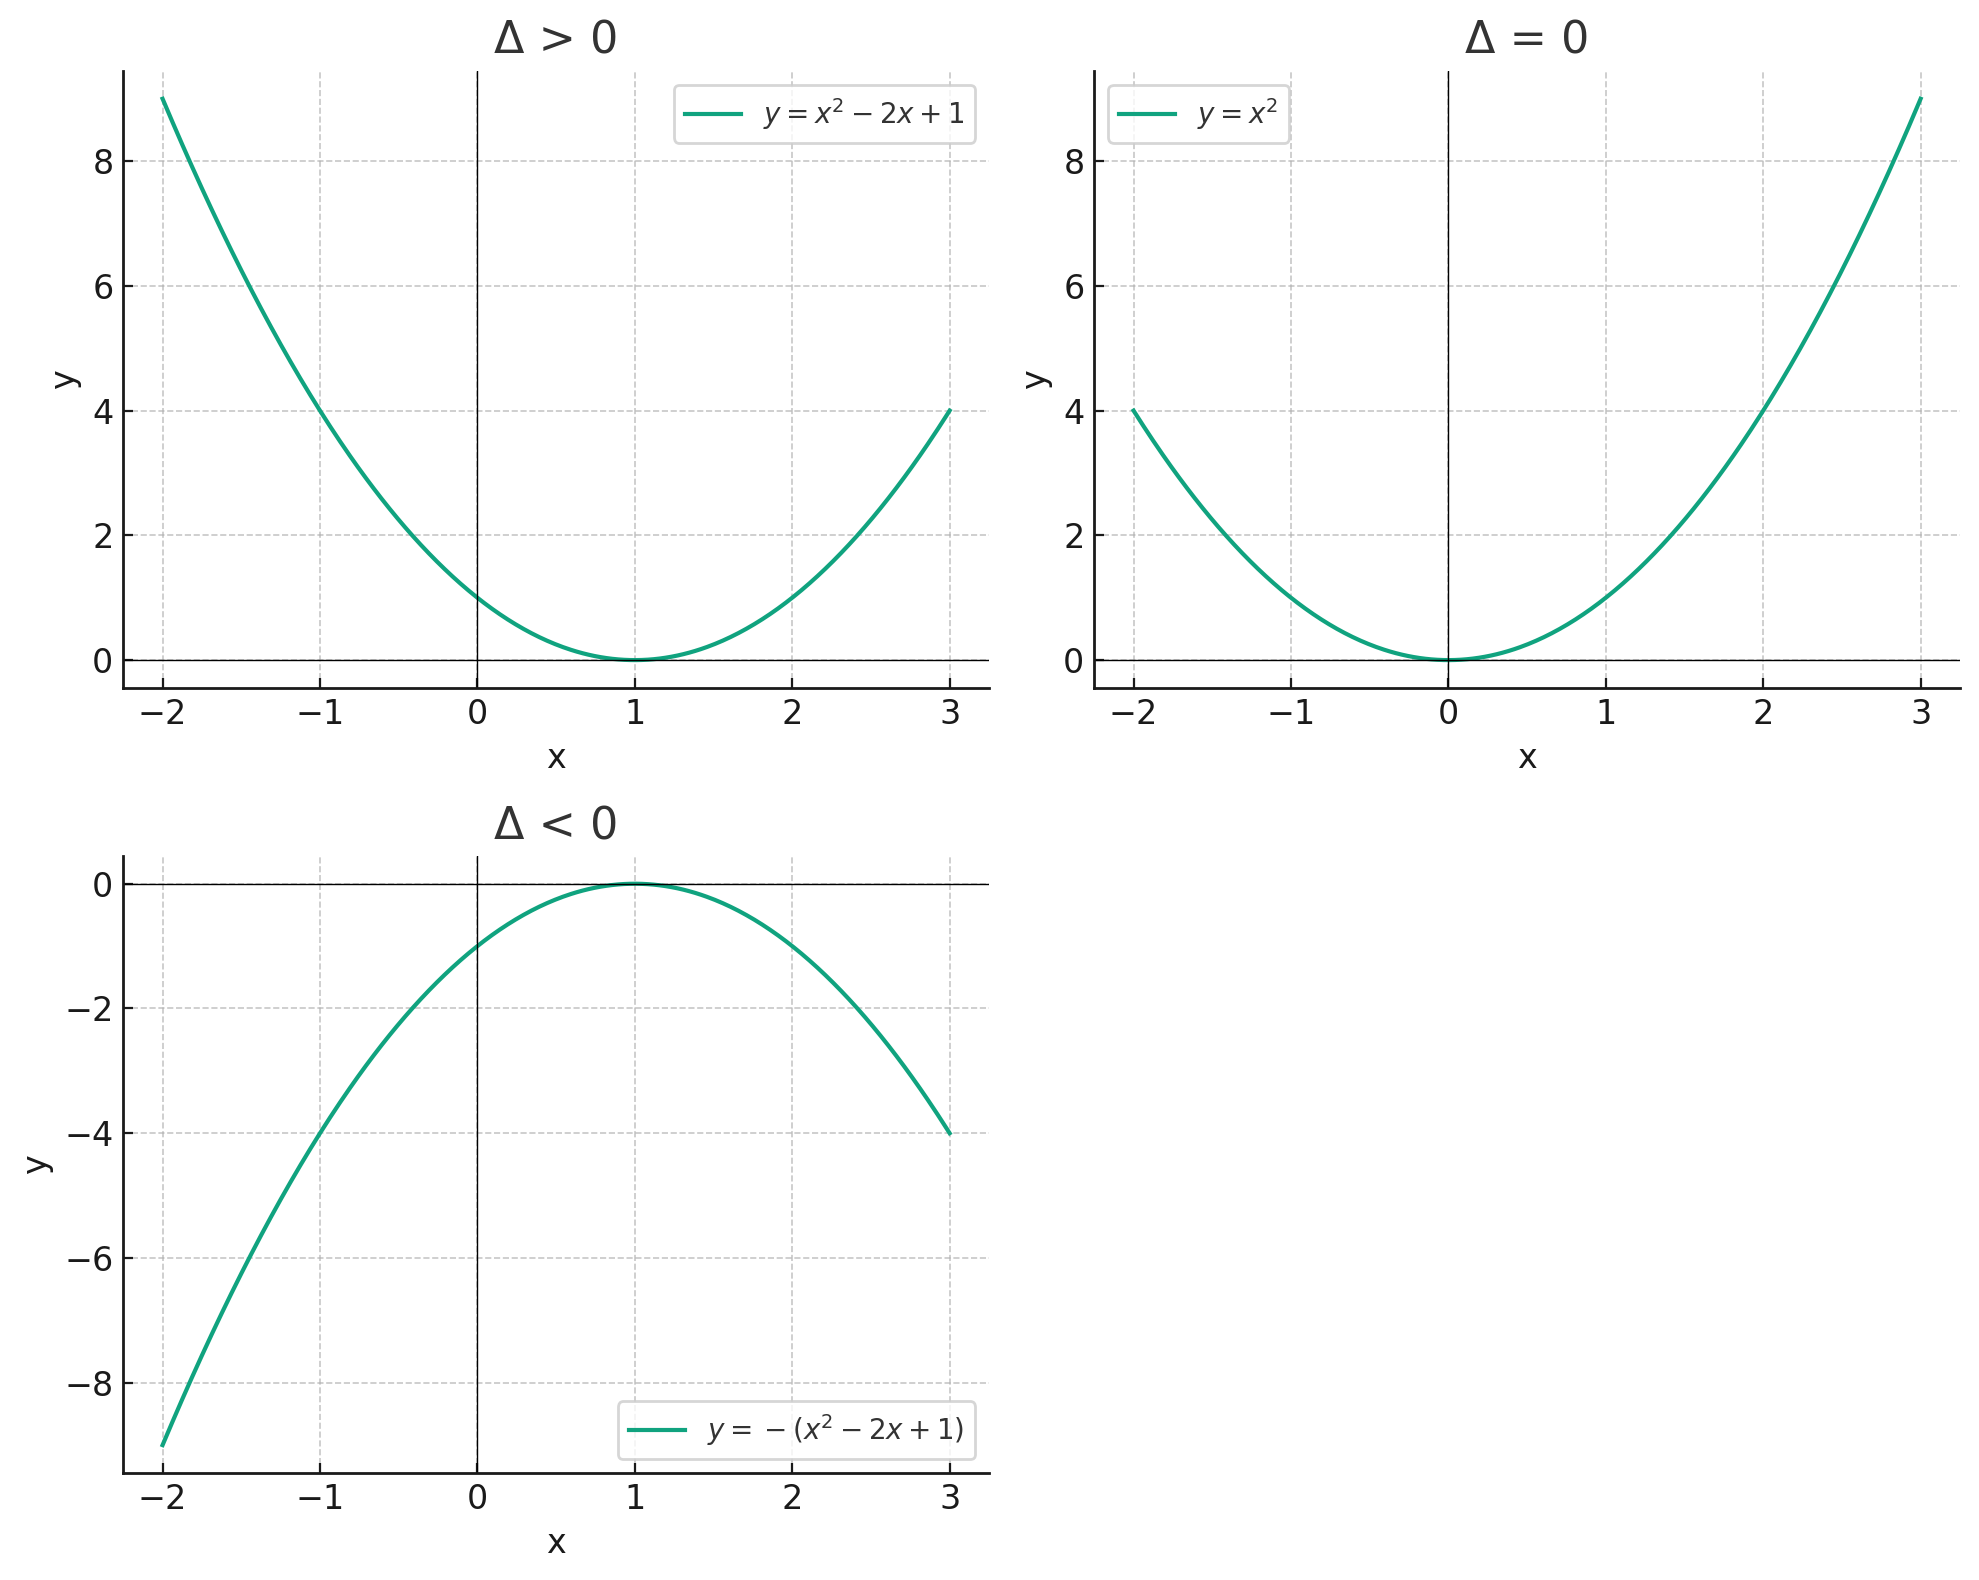
\includegraphics[width=0.8\textwidth]{quadratic.png}
    \caption{Quadratic function graphs based on the discriminant.}
\end{figure}
\begin{example}
    Solve the following quadratic inequalities:

\begin{enumerate}
    \item \(4x^2 + 6x + 2 < 0\);
    \item \(4x^2 + 4x + 1 < 0\);
    \item \(-3x^2 + x - 6 < 0\).
\end{enumerate}
\end{example}
\textbf{Solution:}

\begin{enumerate}
    \item The discriminant \(\Delta = 6^2 - 4 \times 4 \times 2 = 4 > 0\), so the quadratic equation \(4x^2 + 6x + 2 = 0\) has two real roots \(x_1 = -1\), \(x_2 = -\frac{1}{2}\).
    Hence, the solution set for the inequality is \(x \in \left(-\infty, -1\right) \cup \left(-\frac{1}{2}, \infty\right)\).

    \item The discriminant \(\Delta = 4^2 - 4 \times 4 \times 1 = 0\), so the quadratic equation \(4x^2 + 4x + 1 = 0\) has one real double root. Therefore, the inequality has no solution set.

    \item The discriminant \(\Delta = 1^2 - 4 \times (-3) \times (-6) = -71 < 0\), so the quadratic equation \(-3x^2 + x - 6 = 0\) has no real roots.
    Therefore, the solution set for the inequality \(3x^2 - x + 6 > 0\) is all real numbers, and thus the solution set for the given inequality is also all real numbers.
\end{enumerate}

\section{important Inequalities}
In this part, we explore two fundamental inequalities in mathematics: the Triangle Inequality and the Arithmetic-Geometric Mean (AGM) Inequality. Each section provides a comprehensive overview, including detailed proofs and corollaries.
\subsection{The Triangle Inequality}
The Triangle Inequality is a fundamental relation in geometry and analysis, asserting that the sum of the lengths of any two sides of a triangle must be greater than or equal to the length of the remaining side.
    \begin{definition}[Triangular Inequality] \label{triangularineq}
        For any real numbers \( a \) and \( b \), the Triangle Inequality is given by:
        \[ |a + b| \leq |a| + |b| \]
    \end{definition}
    \begin{proof}
        The proof of the Triangle Inequality considers the sign of \( a \) and \( b \):
    \begin{itemize}
     \item \textbf{Case 1:} If \( a \) and \( b \) have the same sign, the inequality follows directly.
        \item \textbf{Case 2:} If \( a \) and \( b \) have opposite signs, assume \( a > 0 \) and \( b < 0      \). Then, \( |a + b| \leq a - b = |a| + |b| \).
    \end{itemize}
    Thus, the Triangle Inequality is proven.
    \end{proof}
    \begin{remark}
        This important inequality will also be seen in other chapters.
    \end{remark}
We also have the following conclusion by preliminary algebra:
$$
\begin{aligned}
    |a{+}b|{\leqslant}|a|+|b|& \Leftrightarrow|a{+}b|^2{\leqslant}(|a|{+}|b|)^2  \\
    &\Leftrightarrow(a+b)^2\leqslant|a|^2+2|a||b|+|b|^2 \\
    &\Leftrightarrow a^2+2ab+b^2\leqslant a^2+2|a|\mid b|+b^2 \\
    &\Leftrightarrow ab{\leqslant}|a|\left|b\right| \\
    &\Leftrightarrow ab\leqslant\lvert ab\rvert.
    \end{aligned}
$$
The quality holds only when $ab \geq 0$.
\subsubsection*{Geometric Explanation of Triangular Inequality}
    Consider $a$ and $b$ are random numbers on a number axis:
    \begin{itemize}
        \item If $ab \geq 0$, then they are both in the same half-axis (both positive or negative). In this case, the distance between $a$ and $-b$
        is the sum of the distance from both points to the origin of the number axis.
        \item  Now consider $ab < 0$, either of them is positive, and the other is negative. In this case, the distance between $a$ and $-b$ is shorter than the sum of 
        the distance from both points to the origin of the number axis.
        \begin{figure}[H]
            \centering
            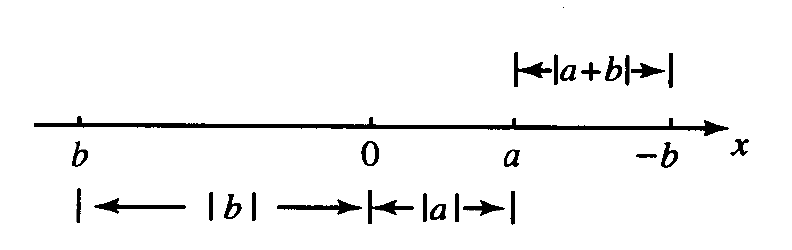
\includegraphics[width = 0.6\textwidth]{triangleablt0.png}
            \caption{Triangular Inequality: $ab < 0$}
        \end{figure}
    \end{itemize}

We also have:
    \begin{theorem}
        For $a, b, c\in \mathbb{R}$, $|a-c|\leq |a-b| + |b-c|$.
    \end{theorem}
    \begin{figure}[H]
        \centering
        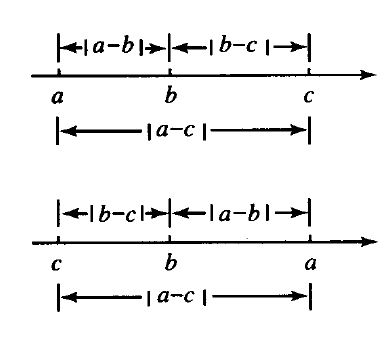
\includegraphics[width = 0.5\textwidth]{triangle2.png}
    \end{figure}
    \begin{proof}
        Since $a-c$, $a-b$, $b-c$ follows the relationship of triangular inequality. We have:
        $$(a-b)(b-c) \geq 0$$
        
        meaning that $b$ is between $a$ and $c$, which could be proven by sketching.
    \end{proof}

    \begin{corollary} \label{trian}
        $||a| - |b|| \leq |a + b|$
    \end{corollary}
    \begin{proof}
        \[ |a| = |(a+b) - b| \leq |a+b| + |-b| = |a+b| + |b|. \]
Therefore,
\[ |a| - |b| \leq |a+b|, \]
and similarly it can be proven that
\[ |b| - |a| \leq |a+b|. \]
Hence,
\[ ||a - b|| \leq |a+b|. \]
    \end{proof}

    \begin{corollary}
        $|a| - |b| \leq |a + b|$
        
    \end{corollary}
    \begin{proof}
        By corollary \autoref{trian}:
        \[ ||a| - |b|| \leq |a + (-b)|, \]
therefore,
\[ ||a| - |-b|| \leq |a - b|. \]
    \end{proof}
%---------------------------------------------------------------------------
    \subsection{The Arithmetic-Geometric Mean Inequality}
    The AGM Inequality(also known as AM-GM inequality) states that for any set of non-negative real numbers, the arithmetic mean is always greater than or equal to the geometric mean.
    \begin{definition}[AGM Inequality] \label{AGM}
        For non-negative real numbers \( a_1, a_2, \ldots, a_n \), the AGM Inequality is:
        \[ \frac{a_1 + a_2 + \cdots + a_n}{n} \geq \sqrt[n]{a_1 \cdot a_2 \cdots a_n} \]
    \end{definition}
    Many methods are available to prove this important conclusion. Below is the proof by MI.
    \begin{proof}
        We prove that for any non-negative real numbers \(x_1, \ldots, x_n\), the following inequality holds:

\[
\alpha^n \geq x_1 x_2 \cdots x_n
\]

where \( \alpha \) is the arithmetic mean of the numbers, with equality if and only if all the numbers are equal.
\begin{remark}
    This is because, the inequality is equivalent to AGM:
    $$\frac{a_{1} +a_{2} +\dotsc +a_{n}}{n} \geq \sqrt[n]{a_{1} \cdot a_{2} \dotsc a_{n}} \Longleftrightarrow \left(\frac{a_{1} +a_{2} +\dotsc +a_{n}}{n}\right)^{n} \geq a_{1} \cdot a_{2} \dotsc a_{n}$$

\end{remark}
\textbf{Induction Basis:}
For \(n = 1\), the statement is trivially true, as the arithmetic mean of a single number is the number itself.

\noindent \textbf{Induction Hypothesis:}
Assume that the AM-GM inequality holds for \(n\) non-negative real numbers.

\noindent \textbf{Induction Step:}
Consider \(n+1\) non-negative real numbers \(x_1, \ldots, x_{n+1}\). Their arithmetic mean \( \alpha \) satisfies:

\[
\alpha = \frac{x_1 + \cdots + x_n + x_{n+1}}{n+1}
\]

If all the \(x_i\) are equal to \( \alpha \), then we have equality in the AM-GM statement, and we are done. In the case where some are not equal to \( \alpha \), there must exist at least one number greater and one smaller than \( \alpha \). Without loss of generality, we can reorder our \(x_i\) to ensure that \(x_n > \alpha > x_{n+1}\), which gives us:
\begin{equation}
    (x_n - \alpha)(\alpha - x_{n+1}) > 0 \label{agm1}
\end{equation}


Define a new number \( y \) with:

\[
y = x_n + x_{n+1} - \alpha \geq x_n - \alpha > 0
\]
Since all numbers from $x_1$ to $y$  are non-negative.

$$\begin{aligned}&(n+1)\alpha=x_1+\cdots+x_{n-1}+x_n+x_{n+1}\\&n\alpha=x_1+\cdots+x_{n-1}+\underbrace{x_n+x_{n+1}-\alpha}_{=y},\end{aligned}$$

This shows that $\alpha$ is also a geometric mean of the n-sequence $x_{1},\ldots,x_{n-1},y$. 

By the induction hypothesis:
$$\alpha^{n+1}=\alpha^n\cdot\alpha\geq x_1x_2\cdots x_{n-1}y\cdot\alpha.$$

From equation \autoref{agm1}, we have:
$$(\underbrace{x_n+x_{n+1}-\alpha}_{=y})\alpha-x_nx_{n+1}=(x_n-\alpha)(\alpha-x_{n+1})>0,$$

Hence:
$$y\cdot \alpha > x_n x_{n+1}$$
By substituting we have:
$$\alpha^{n+1}>x_1x_2\cdots x_{n-1}x_nx_{n+1}$$
This completes the proof.
\end{proof}

\subsubsection*{Geometric representation}
We can use function graphs to visualize the relationship implied in the AGM inequality. On the left and right-hand-side of the inequality sign, there are two functions with $n$ variables.
For simplicity, we use $n=2$ to show its visualization.
We obtain this interactive graph by Mathematica. This simple model involves three variables only. $\displaystyle x_{1}$ and $\displaystyle x_{2}$ are the values to be used to calculate AM and GM. 
We take one of the input value as preimage on the x-axis, and the AM or GM as the image on y-axis. The scroll on the top indicates the value of $\displaystyle x_{2}$. When $\displaystyle x_{2} =0$, the 
graph is shown below. It can be seen that the AGM inequality holds, and only when $\displaystyle x_{2} =x_{1} =0$, there is an intersection$\displaystyle \ ( 0,0) .$

\begin{figure}[H]
    \centering
    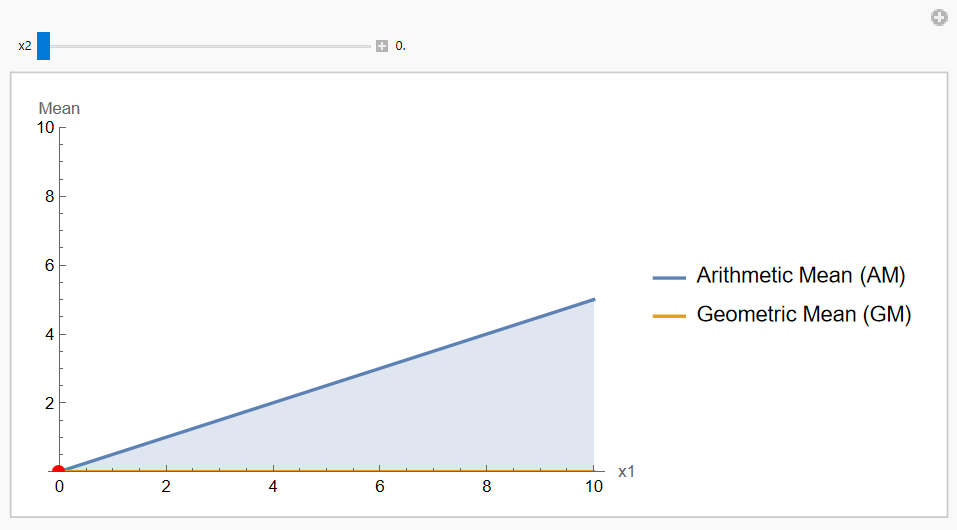
\includegraphics[width=0.8\textwidth]{agmx=0.png}
    \caption{AGM when $x_2 = 0$}
\end{figure}

As we increase the $\displaystyle x_{2}$ value, the GM curve rise up, and the intersection moves on the right direction, remaining on the AM curve. Below is the visualization for $\displaystyle x_{2} =5$. 
There is no any overlap between graphs except the intersection $\displaystyle ( 5,5)$. 

\begin{figure}[H]
    \centering
    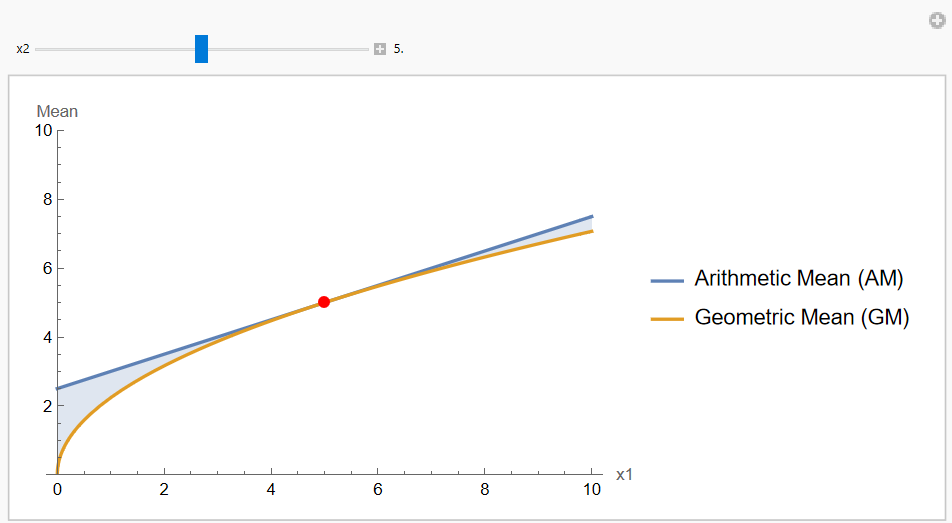
\includegraphics[width=0.8\textwidth]{agmx=5.png}
    \caption{AGM when $x_2 = 5$}
\end{figure}

\begin{problem}
    Where will the intersection go if we have $x_2 = 10$ for this model?
\end{problem}

Now, I think everything is clear, but only things so far. From now on, we will extend the understanding of function graph to a new
dimension, in the 3 dimension space. Functions in the 3D space is extremely important for multi-variable calculus, and learning linear 
algebra also requires us to abstract numbers in more than 3 dimension, but goes up to n dimension space. But don't worry, the discussion
here only involve simple concepts. 

We have three variables: $x_1, x_2, y$, where $y$ is the value of AM or GM from $x_1$ and $x_2$. Coincidently, we have three coordinate
axis in a 3D space. In the three-dimensional coordinate system, we assign two preimages $x_1$, $x_2$ to $x$ and $y$ axis, and the mean
to the $z$ axis. In this way we can get two function graphs, or surface, in the real sense, in the coordinate, which look like in the 
figure below.
\begin{figure}[H]
    \centering
    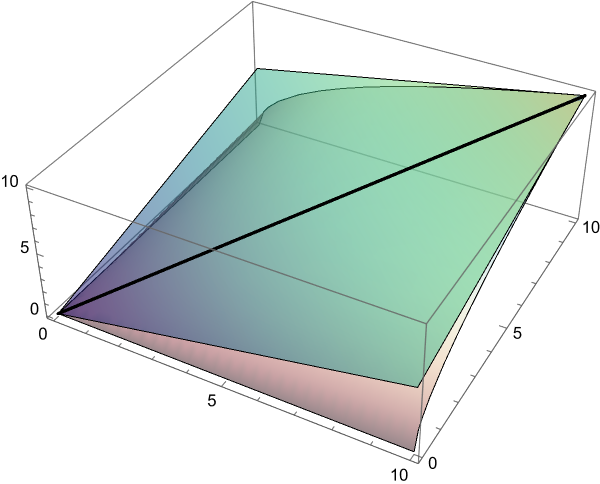
\includegraphics[width=0.6\textwidth]{agm3D.png}
    \caption{AGM 3D Visualization}
\end{figure}

The plane in blue represents the set of all possible arithmetic mean derived from all combinations of $x_1 \text{ and }x_2$ with $x_1,x_2\in [0,10]$, and the other 
surface, almost below the AM plane, is exactly the geometric mean curve that has a similar definition to the former. This is quite different from the functions
we have known, since they are only a line or a curve in the Cartesian coordinate, yet in the 3D coordinate, function could be surface. We will explore more
about multi-variable functions in the future. 

It is noticeable that the two surfaces are actually independent. They intersect in a line that go across the space. That specific line is actually a set of all the
ordered pairs $(x_1,x_2)$ where $x_1 = x_2$. We can actually relate it to the graph in the Cartesian coordinate. If we change the view point to the front of the
curves shaped in the 3D space, we see something like this picture.
\begin{figure}[H]
    \centering
    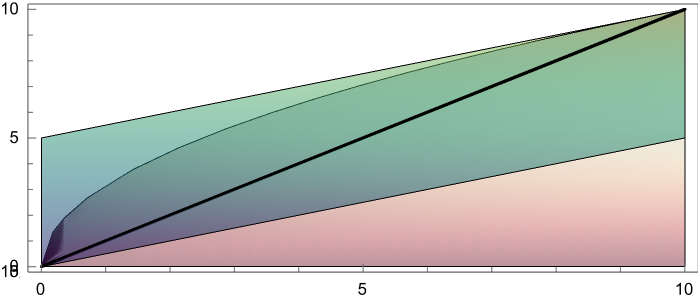
\includegraphics[width=0.6\textwidth]{agm3dsect.png}
    \caption{AGM 3D Visualization (Front)}
\end{figure}
Isn't this quite similar to the 2D graph? Actually, the first image is exactly a horizontal cross-section of the 3D function graph, and the intersection in the 2D 
graph changes as the position of intersection line changes. These explain AGM inequality's geometric meaning.

\subsection*{Conclusions of AGM inequality}
AGM inequality has brought us to these conclusions:
    \begin{corollary}[Mean Inequality Corollary]
If $x, y > 0$, then
\[\frac{2xy}{x+y} \leq \sqrt{xy} \leq \frac{x+y}{2}.\]
Equality holds in each inequality only when $x = y$.
\end{corollary}

\begin{proof}
Proposition \ref{AGM} yields $\sqrt{xy} \leq \frac{x+y}{2}$. We obtain the other inequality from this by multiplying both sides by the positive number $\frac{2\sqrt{xy}}{x+y}$, leading to:
\[\sqrt{xy} \cdot \frac{2\sqrt{xy}}{x+y} \leq \frac{x+y}{2} \cdot \frac{2\sqrt{xy}}{x+y},\]
which simplifies to:
\[\frac{2xy}{x+y} \leq \sqrt{xy}.\]
Thus, we have shown that $\frac{2xy}{x+y} \leq \sqrt{xy} \leq \frac{x+y}{2}$, with equality if and only if $x = y$.
\end{proof}
The expression $\frac{2xy}{x+y}$ is the harmonic mean of $x$ and $y$. It arises in the study of average rates. For example, consider traveling a distance $d$ at rate $r_1$ in time $t_1$ and making the return trip at rate $r_2$ in time $t_2$. The harmonic mean gives us the average rate $r$ for the full trip.

Assuming we travel the same distance $d$ for both trips, we have:
\begin{align*}
r_1t_1 &= d \\
r_2t_2 &= d
\end{align*}

The average rate $r$ for the full trip is computed as follows:
\begin{align*}
r &= \frac{2d}{t_1 + t_2} = \frac{2d}{\frac{d}{r_1} + \frac{d}{r_2}} = \frac{2d}{\frac{r_1r_2(t_1 + t_2)}{r_1r_2}} =\frac{2r_1r_2}{r_1 + r_2}\\
\end{align*}

The other important corollary of AGM inequality is:
\begin{corollary}
    $a^2+b^2 \geq 2ab$
\end{corollary}
\begin{proof}
    $a^2 + b^2 \geq 2ab \iff a^2 + b^2 - 2ab \geq 0 \iff (a - b)^2 \geq 0.$
\end{proof}


\subsection{Exercises}
\begin{exercise}
    Prove that for any triangle with sides \(a\), \(b\), and \(c\), the following inequality holds:
\[ \frac{a}{b + c} + \frac{b}{a + c} + \frac{c}{a + b} > 1 \]
\end{exercise}
\begin{proof}

Given a triangle with sides \(a\), \(b\), and \(c\), we know that for any triangle, the sum of the lengths of any two sides is greater than the length of the third side. Therefore, \(a < b + c\), \(b < a + c\), and \(c < a + b\).

Now, consider the inequality \(\frac{a}{b + c} > \frac{a}{a + b + c}\). This is true because \(b + c > a\) implies that the denominator of the left-hand side is smaller than that of the right-hand side while keeping the numerator constant.

Similarly, we can show that \(\frac{b}{a + c} > \frac{b}{a + b + c}\) and \(\frac{c}{a + b} > \frac{c}{a + b + c}\).

Adding these three inequalities, we get:
\[ \frac{a}{b + c} + \frac{b}{a + c} + \frac{c}{a + b} > \frac{a + b + c}{a + b + c} \]

Simplifying the right-hand side, we obtain:
\[ \frac{a}{b + c} + \frac{b}{a + c} + \frac{c}{a + b} > 1 \]

Thus, the inequality is proven. 

\end{proof}

\begin{exercise}
    Given $\varepsilon > 0$, if $|x - a| < \frac{\varepsilon}{4}$ and $|y - b| < \frac{\varepsilon}{6}$, prove that:

\[
|2x + 3y - 2a - 3b| < \varepsilon.
\]
\end{exercise}
Hint: Rearrange it in a form that is good for using triangle inequality.
\begin{proof}
    \begin{align*}
        |2x + 3y - 2a - 3b| &= |2(x - a) + 3(y - b)| \\
        &\leq |2(x - a)| + |3(y - b)| \\
        &= 2|x - a| + 3|y - b| \\
        &< 2 \times \frac{\varepsilon}{4} + 3 \times \frac{\varepsilon}{6} \\
        &= \varepsilon.
        \end{align*}
\end{proof}

\begin{exercise}
    Prove for any real numbers \( a, b, c, d \) that:
\[ |a - b| + |b - c| + |c - d| + |d - a| \geq |a - c| + |b - d| \]

\end{exercise}

\begin{proof}
    \begin{enumerate}
    \item \textbf{Application of the Triangle Inequality:}
    The triangle inequality states that for any real numbers \( x, y, z \):
    \[ |x - y| \leq |x - z| + |z - y| \]
    We can apply this inequality to certain terms in our original problem. For example, consider \( |a - c| \) and \( |b - d| \).

    \item \textbf{Separate Applications of the Triangle Inequality:}
    For \( |a - c| \), we have:
    \[ |a - c| \leq |a - b| + |b - c| \]
    For \( |b - d| \), we have:
    \[ |b - d| \leq |b - c| + |c - d| \]

    \item \textbf{Combining Inequalities:}
    Adding the above two inequalities, we get:
    \[ |a - c| + |b - d| \leq |a - b| + 2|b - c| + |c - d| \]

    \item \textbf{Simplification and Rearrangement:}
    Notice that \( 2|b - c| \) appears on the right side of the inequality. However, since \( |b - c| \) is non-negative, we can remove one \( |b - c| \) and the inequality still holds. Hence, we have:
    \[ |a - c| + |b - d| \leq |a - b| + |b - c| + |c - d| \]
    This is the reverse of the inequality in our original problem, so we can conclude:
    \[ |a - b| + |b - c| + |c - d| + |d - a| \geq |a - c| + |b - d| \]

    \item \textbf{Conclusion:}
    Therefore, the original inequality is proved.
\end{enumerate}
\end{proof}
\begin{exercise}
    Prove that for any real numbers \( x, y, z \), the following inequality holds:
\[ |x + y + z| \leq |x| + |y| + |z| \]

\end{exercise}
\begin{proof}
    We will use the triangle inequality which states that for any real numbers \( a \) and \( b \):
\[ |a + b| \leq |a| + |b| \]

First, apply the triangle inequality to \( x \) and \( y \):
\[ |x + y| \leq |x| + |y| \]

Now, let \( a = x + y \) and \( b = z \), and apply the triangle inequality again:
\[ |(x + y) + z| \leq |x + y| + |z| \]

Substitute the first inequality into the second one:
\[ |x + y + z| \leq |x| + |y| + |z| \]

This completes the proof.
\end{proof}
\begin{exercise}
    Prove that for any sequence of real numbers \( x_1, x_2, \ldots, x_n \), the following inequality holds:
\[ \left|x_1 + x_2 + \ldots + x_n\right| \leq \left|x_1\right| + \left|x_2\right| + \ldots + \left|x_n\right| \]
\end{exercise}
\begin{proof}
    We will prove this by induction on the number of terms \( n \).

\textit{Base case} (\( n = 1 \)):
For a single real number \( x_1 \), the inequality trivially holds as:
\[ \left|x_1\right| = \left|x_1\right| \]

\textit{Inductive step}:
Assume the inequality holds for some \( n = k \), i.e.,
\[ \left|x_1 + x_2 + \ldots + x_k\right| \leq \left|x_1\right| + \left|x_2\right| + \ldots + \left|x_k\right| \]
Now, consider the case when \( n = k + 1 \). By the triangle inequality, we have:
\[ \left|x_1 + x_2 + \ldots + x_k + x_{k+1}\right| \leq \left|x_1 + x_2 + \ldots + x_k\right| + \left|x_{k+1}\right| \]

Using the induction hypothesis, we can then write:
\[ \left|x_1 + x_2 + \ldots + x_k + x_{k+1}\right| \leq \left(\left|x_1\right| + \left|x_2\right| + \ldots + \left|x_k\right|\right) + \left|x_{k+1}\right| \]
\[ \left|x_1 + x_2 + \ldots + x_k + x_{k+1}\right| \leq \left|x_1\right| + \left|x_2\right| + \ldots + \left|x_k\right| + \left|x_{k+1}\right| \]

This completes the inductive step and thus, by the principle of mathematical induction, the inequality holds for all positive integers \( n \).
\end{proof}

\begin{exercise}
    Let \(a\), \(b\), \(c\) be positive real numbers. Prove the inequality:
\[ (a+b+c)(a^2+b^2+c^2) > 9abc. \]
\end{exercise}
\begin{proof}
    By the Arithmetic Mean-Geometric Mean Inequality (AM-GM Inequality), we have:
\[ \frac{a^2+b^2+c^2}{3} \geq \sqrt[3]{a^2b^2c^2}, \]
\[ \frac{a+b+c}{3} \geq \sqrt[3]{abc}. \]

Cubing both sides of the inequalities, we get:
\[ (a^2+b^2+c^2)^3 \geq 27a^2b^2c^2, \]
\[ (a+b+c)^3 \geq 27abc. \]

Multiplying the resulting inequalities, we obtain:
\[ (a^2+b^2+c^2)^3(a+b+c)^3 \geq (27a^2b^2c^2)(27abc). \]

Taking the cube root of both sides, we arrive at:
\[ (a^2+b^2+c^2)(a+b+c) \geq 9abc. \]

Note that the inequality is strict when \(a\), \(b\), \(c\) are positive real numbers, thus:
\[ (a^2+b^2+c^2)(a+b+c) > 9abc. \]
\end{proof}

\begin{exercise}
    Given non-negative real numbers \( a, b, c \) such that \( a + b + c = 1 \), we want to prove that:
\[ a^2 + b^2 + c^2 \geq \frac{1}{3}. \]
\end{exercise}
\begin{proof}
    We will use the Arithmetic Mean-Geometric Mean Inequality (AM-GM Inequality) which states that for any non-negative real numbers \( x, y, z \), the following holds:
\[ \frac{x + y + z}{3} \geq \sqrt[3]{xyz}. \]

Applying this to \( a, b, c \), we have:
\[ \frac{a + b + c}{3} \geq \sqrt[3]{abc} \Rightarrow \frac{1}{3} \geq \sqrt[3]{abc}. \]

Cubing both sides of the inequality yields:
\[ \frac{1}{27} \geq abc. \]

Now, by AM-GM applied to \( a^2, b^2, c^2 \), we get:
\[ \frac{a^2 + b^2 + c^2}{3} \geq \sqrt[3]{a^2b^2c^2}. \]

Since \( a^2b^2c^2 \) is the square of \( abc \), it follows that:
\[ \frac{a^2 + b^2 + c^2}{3} \geq (abc)^{\frac{2}{3}}. \]

Given \( \frac{1}{27} \geq abc \), we have:
\[ (abc)^{\frac{2}{3}} \leq \left(\frac{1}{27}\right)^{\frac{2}{3}} = \frac{1}{9}. \]

Therefore, we can conclude that:
\[ \frac{a^2 + b^2 + c^2}{3} \geq \frac{1}{9}. \]

Multiplying through by 3, we obtain the desired inequality:
\[ a^2 + b^2 + c^2 \geq \frac{1}{3}. \]

Hence, we have proved that \( a^2 + b^2 + c^2 \geq \frac{1}{3} \) as required.
\end{proof}

\begin{exercise}
    Consider the function
    \[
    f(x, y, z) = \frac{x}{y} + \frac{y}{z} + \frac{z}{x}
    \]
    for all positive real numbers \( x, y, \) and \( z \). Find the minimal value of the function.
    \end{exercise}
    
    \begin{proof}
    For \( (x, y, z) \) positive real numbers, we have
    \[
    f(x, y, z) = \frac{x}{y} + \frac{y}{z} + \frac{z}{x}
    \]
    can be rewritten as
    \[
    f(x, y, z) = 6 \cdot \left( \frac{1}{6} \cdot \frac{x}{y} + \frac{1}{6} \cdot \frac{y}{z} + \frac{1}{6} \cdot \frac{z}{x} + \frac{1}{6} \cdot \frac{x}{y} + \frac{1}{6} \cdot \frac{y}{z} + \frac{1}{6} \cdot \frac{z}{x} \right)
    \]
    Setting \( x_1 = \frac{x}{y}, x_2 = x_3 = \frac{1}{2} \cdot \frac{y}{z}, x_4 = x_5 = x_6 = \frac{1}{3} \cdot \frac{z}{x} \), and applying the AM-GM inequality for \( n = 6 \), we get
    \[
    f(x, y, z) \geq 6 \cdot \sqrt[6]{x_1 \cdot x_2 \cdot x_3 \cdot x_4 \cdot x_5 \cdot x_6} = 6 \cdot \sqrt[6]{\frac{1}{2 \cdot 2 \cdot 3 \cdot 3 \cdot 3} \cdot \frac{x}{y} \cdot \frac{y}{z} \cdot \frac{z}{x}}
    \]
    which simplifies to
    \[
    f(x, y, z) \geq 6 \cdot \sqrt[6]{\frac{1}{2^2 \cdot 3^3}} = 2^{2/3} \cdot 3^{1/2}
    \]
    Further, we know that the two sides are equal exactly when all the terms of the mean are equal. Thus,
    \[
    f(x, y, z) = 2^{2/3} \cdot 3^{1/2}
    \]
    when
    \[
    \frac{x}{y} = \frac{1}{2} \cdot \frac{y}{z} = \frac{1}{3} \cdot \frac{z}{x}
    \]
    All the points \( (x, y, z) \), satisfying these conditions lie on a half-line starting at the origin and are given by,
    \[
    (x, y, z) = \left( t, \frac{3}{2}\sqrt{3}t, \frac{3}{2}\sqrt{3}t \right)
    \]
    with \( t > 0 \).
    \end{proof}
    
%------------------------------------------------
\subsection{Cauchy-Schwarz Inequality}
Cauchy-Schwarz inequality is another important inequality that is used for mathematical proofs. 

\begin{theorem}[Cauchy-Schwarz Inequality]\label{CSineq}
    Let \( a_1, \ldots, a_n \) and \( b_1, \ldots, b_n \) be real numbers. Then
\[
(a_1b_1 + a_2b_2)^2 \leq (a_1^2 + a_2^2)(b_1^2 + b_2^2)
\]
\end{theorem}
\begin{proof}
\[
(a_1 + a_2)(b_1^2 + b_2^2) - (a_1b_1 + a_2b_2)^2 \geq 0
\]
\[
\Leftrightarrow a_1^2b_1^2 + a_2^2b_2^2 + a_1^2b_2^2 + a_2^2b_1^2 - a_1^2b_1^2 - a_2^2b_2^2 - 2a_1a_2b_1b_2 \geq 0
\]
\[
\Leftrightarrow a_1^2b_2^2 - 2a_1a_2b_1b_2 + a_2^2b_1^2 \geq 0
\]
\[
\Leftrightarrow (a_1b_2 - a_2b_1)^2 \geq 0
\]
Hence, the equality holds if an only if when $a_1b_2=a_2b_1$.
\end{proof}

This is not a difficult proof, but it does not show all the implications of the inequality, especially in
geometry. Let's take a look at how we can derive its vector form.

In the inequality of the inner product in vector space, let \(\alpha\) and \(\beta\) be the directed line segments determined by vectors \(\mathbf{a}\) and \(\mathbf{b}\) respectively, with terminal coordinates \(a_1, a_2\) and \(b_1, b_2\), and let
\[
\alpha = (a_1, a_2), \quad \beta = (b_1, b_2),
\]
Then, \(\alpha\) and \(\beta\) are not both zero, and the angle between them is denoted as \(\langle \alpha, \beta \rangle\), with the convention that
\[
0 \leq \langle \alpha, \beta \rangle \leq \pi.
\]
The \(\cos \langle \alpha, \beta \rangle\) is called the cosine of the angle (inner product) between vectors \(\alpha\) and \(\beta\), denoted as \(\alpha \cdot \beta\), and
\[
\alpha \cdot \beta = a_1b_1 + a_2b_2,
\]
\[
|\alpha| = \sqrt{\alpha \cdot \alpha} = \sqrt{a_1^2 + a_2^2},
\]
\[
|\beta| = \sqrt{\beta \cdot \beta} = \sqrt{b_1^2 + b_2^2},
\]
Therefore,
\[
\cos\langle \alpha, \beta \rangle = \frac{a_1b_1 + a_2b_2}{\sqrt{a_1^2 + a_2^2} \sqrt{b_1^2 + b_2^2}},
\]
\[
\cos^2\langle \alpha, \beta \rangle = \left(\frac{a_1b_1 + a_2b_2}{\sqrt{a_1^2 + a_2^2} \sqrt{b_1^2 + b_2^2}}\right)^2 \leq 1,
\]
which implies
\[
(a_1^2 + a_2^2)(b_1^2 + b_2^2) \geq (a_1b_1 + a_2b_2)^2,
\]
and since
\begin{equation}\label{CSvec}
    \sqrt{a_1^2 + a_2^2} \sqrt{b_1^2 + b_2^2} \geq |a_1b_1 + a_2b_2|.
\end{equation}

It is evident that \(\cos^2\langle \alpha, \beta \rangle = 1\) implies \(\langle \alpha, \beta \rangle = 0\) or \(\pi\), which corresponds to vectors \(\alpha\) and \(\beta\) being parallel or anti-parallel. When the angle is 0, vectors A and B are in the same direction, which is the condition for equality.

\begin{theorem}[Cauchy-Schwarz Inequality(vector)]
    \label{CSvector}
    Assume that $\alpha = (a_1, a_2)$ and $\beta = (b_1, b_2)$ are two planar vectors, then
    $$|\alpha||\beta|\geq |\alpha \cdot \beta|$$
    and$$\sqrt{a_1^2 + a_2^2} \sqrt{b_1^2 + b_2^2} \geq |a_1b_1 + a_2b_2|$$
\end{theorem}   

It is noticeable that when we take $a_2=b_2=0$, we have
$$|a_1|+|b_1|\geq|a_1+b_1|$$
which is exactly the triangle inequality for vector that we have discussed earlier.


%------------------------------------------------
\subsection{Rearrangement Inequality}
This section introduces \textbf{Rearrangement Inequality}, whose direct conclusions are the \href{https://en.wikipedia.org/wiki/QM-AM-GM-HM_Inequalities}{QM-AM-GM-HM inequality}.

We start with an example. Suppose there are four boxes containing \$10, \$20, \$50 and \$100 bills, respectively. You may take 2 bills from one box, 3 bills from another, 4 bills from another, and 5 bills from the remaining box. What is the maximum amount of money you can get?

Clearly, you’d want to take as many bills as possible from the box with largest-value bills! So you would take 5 \$100 bills, 4 \$50 bills, 3 \$20 bills, and 2 \$10 bills, for a grand total of
\begin{equation}\label{eq4.3}
5 \cdot \$100 + 4 \cdot \$50 + 3 \cdot \$20 + 2 \cdot \$10 = \$780.
\end{equation}

Suppose instead that your arch-nemesis (who isn't very good at math) is picking the bills instead, and he asks you how many bills he should take from each box. In this case, to minimize the amount of money he gets, you’d want him to take as many bills as possible from the box with lowest-value bills. So you tell him to take 5 \$10 bills, 4 \$20 bills, 3 \$50 bills, and 2 \$100 bills, for a grand total of
\begin{equation}\label{eq4.4}
5 \cdot \$10 + 4 \cdot \$20 + 3 \cdot \$50 + 2 \cdot \$100 = \$480.
\end{equation}

The maximum is attained when the number of bills taken and the denominations are similarly sorted as
 in Eq. \ref{eq4.3} and the minimum is attained when they are oppositely sorted as in \ref{eq4.4}. The Rearrangement Inequality formalizes this observation.
\begin{theorem}{Rearrangement}
    Let \( x_1, x_2, \ldots, x_n \) and \( y_1, y_2, \ldots, y_n \) be real numbers (not necessarily positive) with
\[ x_1 \leq x_2 \leq \ldots \leq x_n, \quad \text{and} \quad y_1 \leq y_2 \leq \ldots \leq y_n, \]
and let \( \sigma \) be a permutation of \( \{1, 2, \ldots, n\} \). (That is, \( \sigma \) sends each of \( 1, 2, \ldots, n \) to a different value in \( \{1, 2, \ldots, n\} \).) Then the following inequality holds:
\[ x_1y_n + x_2y_{n-1} + \ldots + x_ny_1 \leq x_1y_{\sigma(1)} + x_2y_{\sigma(2)} + \ldots + x_ny_{\sigma(n)} \leq x_1y_1 + x_2y_2 + \ldots + x_ny_n. \]
\end{theorem}
\begin{proof}
    We prove the inequality on the right by induction on \( n \). The statement is obvious for \( n = 1 \). Suppose it true for \( n - 1 \). Let \( m \) be an integer such that \( \sigma(m) = n \). Since
\[ x_n \geq x_m \quad \text{and} \quad y_n \geq y_{\sigma(n)}, \]
we have
\[ 0 \leq (x_n - x_m)(y_n - y_{\sigma(n)}) \quad \]
\[\implies x_my_n + x_ny_{\sigma(n)} \leq x_my_{\sigma(n)} + x_ny_n. \]

Hence
\[ x_1y_{\sigma(1)} + \ldots + x_my_{\sigma(m)} + \ldots + x_ny_{\sigma(n)} \leq x_1y_{\sigma(1)} + \ldots + x_my_n + \ldots + x_ny_n. \]

By the induction hypothesis,
\[ x_1y_{\sigma(1)} + \ldots + x_my_n + \ldots + x_ny_{\sigma(n-1)} \leq x_1y_1 + \ldots + x_my_m + \ldots + x_ny_{n-1}. \]

Thus the RHS is at most \( x_1y_1 + \ldots + x_{n-1}y_{n-1} + x_ny_n \), as needed.
To prove the LHS, apply the above with \( -y_i \) instead of \( y_i \) (noting that negating an inequality reverses the sign).
\end{proof}
\begin{remark}
    The equality holds if and only if $a_1 = a_2 =\cdots a_n$ or $b_1 = b_2 =\cdots b_n$
\end{remark}
%------------------------------------------------
\subsection{Exercises}
\begin{exercise}
    Prove that for any real numbers \( a \), \( b \), \( c \), and \( d \), the following inequality holds:
    \[
    a^2 + b^2 + c^2 + d^2 \geq ab + bc + cd + da.
    \]
\end{exercise}
\begin{proof}
    Consider the sequences \( (a, b, c, d) \) and \( (b, c, d, a) \). By the Cauchy-Schwarz inequality, we have:
    \[
    (a^2 + b^2 + c^2 + d^2)(b^2 + c^2 + d^2 + a^2) \geq (ab + bc + cd + da)^2.
    \]
    $$\left(a^2+b^2+c^2+d^2\right)^2 \geq (ab + bc + cd + da)^2$$
    \[
    a^2 + b^2 + c^2 + d^2 \geq ab + bc + cd + da.
    \]
    This completes the proof.
\end{proof}
\begin{exercise}
    In mathematics, the QM-AM-GM-HM inequalities, also known as the mean inequality chain, state the relationship between the harmonic mean, geometric mean, arithmetic mean, and quadratic mean (also known as root mean square).
    It follows that:
    \begin{equation}
        0<\frac{n}{\frac{1}{x_{1}}+\frac{1}{x_{2}}+\cdots+\frac{1}{x_{n}}} \leq \sqrt[n]{x_{1} x_{2} \cdots x_{n}} \leq \frac{x_{1}+x_{2}+\cdots+x_{n}}{n} \leq \sqrt{\frac{x_{1}^{2}+x_{2}^{2}+\cdots+x_{n}^{2}}{n}}
    \end{equation}
    The right part of the inequality is a direct conclusion from Cauchy-Schwarz inequality. Prove it by
    substituting special values to fit the relation.
\end{exercise}
\begin{proof}
    Cauchy-Schwarz inequality states that:
    $$\left(a_{1}^{2}+a_{2}^{2}+\cdots+a_{n}^{2}\right)\left(b_{1}^{2}+b_{2}^{2}+\cdots+b_{n}^{2}\right) \geq\left(a_{1} b_{1}+a_{2} b_{2}+\cdots+a_{n} b_{n}\right)^{2}$$
    where all terms are real numbers.
    Let $b_1=b_2=\cdots=b_n=1$, we have:
    $$\left(x_{1}^{2}+x_{2}^{2}+\cdots+x_{n}^{2}\right)(1+1+\cdots+1) \geq\left(x_{1}+x_{2}+\cdots+x_{n}\right)^{2}$$

    $$\frac{x_{1}^{2}+x_{2}^{2}+\cdots+x_{n}^{2}}{n} \geq\left(\frac{x_{1}+x_{2}+\cdots+x_{n}}{n}\right)^{2}$$
    $$\sqrt{\frac{x_{1}^{2}+\cdots+x_{n}^{2}}{n}} \geq \frac{x_{1}+\cdots+x_{n}}{n}$$
    This completes the proof.
\end{proof}
If you are interested in the complete proof, check \href{https://artofproblemsolving.com/wiki/index.php/Root-Mean_Square-Arithmetic_Mean-Geometric_Mean-Harmonic_mean_Inequality}{this link}.
\begin{exercise}
    Prove that, let \( a, b, c \) be positive real numbers such that \( a + b + c = 1 \). Then the following inequality holds:
\[
\frac{1}{a} + \frac{1}{b} + \frac{1}{c} \geq 9.
\]
\end{exercise}
\begin{proof}
    By applying the Cauchy-Schwarz inequality to the sequences \( (\sqrt{a}, \sqrt{b}, \sqrt{c}) \) and \( (\frac{1}{\sqrt{a}}, \frac{1}{\sqrt{b}}, \frac{1}{\sqrt{c}} ) \), we have:
\[
\left( (\sqrt{a})^2 + (\sqrt{b})^2 + (\sqrt{c})^2 \right) \left( \left(\frac{1}{\sqrt{a}}\right)^2 + \left(\frac{1}{\sqrt{b}}\right)^2 + \left(\frac{1}{\sqrt{c}}\right)^2 \right) 
\]
\[
\geq \left( \sqrt{a} \cdot \frac{1}{\sqrt{a}} + \sqrt{b} \cdot \frac{1}{\sqrt{b}} + \sqrt{c} \cdot \frac{1}{\sqrt{c}} \right)^2
\]
Simplifying both sides of the inequality gives us:
\[
(a + b + c) \left( \frac{1}{a} + \frac{1}{b} + \frac{1}{c} \right) \geq (1 + 1 + 1)^2
\]
Given that \( a + b + c = 1 \), substituting this into the inequality yields:
\[
1 \cdot \left( \frac{1}{a} + \frac{1}{b} + \frac{1}{c} \right) \geq 3^2
\]
Therefore, we have:
\[
\frac{1}{a} + \frac{1}{b} + \frac{1}{c} \geq 9.
\]
This completes the proof.
\end{proof}
\begin{exercise}
    We have proven the Cauchy-Schwarz inequality for planar vectors, can you expand theorem \ref{CSvector}
to 3D vectors? Hint: Express your solution in the form of Eq. \ref{CSvec}. No extra thinking is needed.
\end{exercise}
\textbf{Solution:}

In the 3D space, we have
\begin{corollary}
    Assume that $\alpha = (a_1, a_2, a_3)$ and $\beta = (b_1, b_2, b_3)$ are two 3D vectors:
    \[
\sqrt{a_1^2 + a_2^2 + a_3^2}\sqrt{b_1^2 + b_2^2 + b_3^2} \geq |a_1b_1 + a_2b_2 + a_3b_3|.
\] 
\end{corollary}
\begin{proof}
    In the inequality of the inner product in vector space, let \( \alpha \) and \( \beta \) be the directed line segments determined by vectors \(\mathbf{a}\) and \(\mathbf{b}\) respectively, with terminal coordinates \( a_1, a_2, a_3 \) and \( b_1, b_2, b_3 \), and let
\[
\alpha = (a_1, a_2, a_3), \quad \beta = (b_1, b_2, b_3),
\]
Then, \( \alpha \) and \( \beta \) are not both zero, and the angle between them is denoted as \( \langle \alpha, \beta \rangle \), with the convention that
\[
0 \leq \langle \alpha, \beta \rangle \leq \pi.
\]
The \( \cos\langle \alpha, \beta \rangle \) is called the cosine of the angle (inner product) between vectors \( \alpha \) and \( \beta \), denoted as \( \alpha \cdot \beta \), and
\[
\alpha \cdot \beta = a_1b_1 + a_2b_2 + a_3b_3,
\]
\[
|\alpha| = \sqrt{\alpha \cdot \alpha} = \sqrt{a_1^2 + a_2^2 + a_3^2},
\]
\[
|\beta| = \sqrt{\beta \cdot \beta} = \sqrt{b_1^2 + b_2^2 + b_3^2},
\]
Therefore,
\[
\cos\langle \alpha, \beta \rangle = \frac{a_1b_1 + a_2b_2 + a_3b_3}{\sqrt{a_1^2 + a_2^2 + a_3^2}\sqrt{b_1^2 + b_2^2 + b_3^2}},
\]
\[
\cos^2\langle \alpha, \beta \rangle = \left(\frac{a_1b_1 + a_2b_2 + a_3b_3}{\sqrt{a_1^2 + a_2^2 + a_3^2}\sqrt{b_1^2 + b_2^2 + b_3^2}}\right)^2 \leq 1,
\]
which implies
\[
(a_1^2 + a_2^2 + a_3^2)(b_1^2 + b_2^2 + b_3^2) \geq (a_1b_1 + a_2b_2 + a_3b_3)^2,
\]
and since
\[
\sqrt{a_1^2 + a_2^2 + a_3^2}\sqrt{b_1^2 + b_2^2 + b_3^2} \geq |a_1b_1 + a_2b_2 + a_3b_3|.
\]
which completes the proof.
\end{proof}
\begin{exercise}
    We have shown that the Cauchy-Schwarz inequality still works in the 3-dimensional space, why not try
    to show that it holds for all vectors in the n-dimension space? Think about the strategy to be used and show your 
    meticulous proof for nD vector. Hint: We are actually trying to find a generalized form of the inequality.
    Try to express it in an open form (summation).
\end{exercise}
\textbf{Solutions:}
\begin{theorem}[Generalized Cauchy-Schwarz Inequality(vector)]\label{gcsineq}
    We consider vectors in n-dimentional space.
    Let \( \mathbf{a} = (a_1, a_2, \ldots, a_n) \) and \( \mathbf{b} = (b_1, b_2, \ldots, b_n) \) be two \( n \)-dimensional vectors. Then the following inequality holds:
\[
\left(\sum_{i=1}^{n} a_i b_i\right)^2 \leq \left(\sum_{i=1}^{n} a_i^2\right) \left(\sum_{i=1}^{n} b_i^2\right)
\]
\end{theorem}
\begin{proof}
    We will prove the Cauchy-Schwarz inequality for \( n \)-dimensional vectors using mathematical induction.

\textbf{Base Case:} For \( n = 1 \), we have:
\[
(a_1b_1)^2 \leq (a_1^2)(b_1^2)
\]
which is obviously true, as both sides are equal.

\textbf{Inductive Step:}
Assume the inequality holds for \( n = k \), that is:
\[
\left(\sum_{i=1}^{k} a_ib_i\right)^2 \leq \left(\sum_{i=1}^{k} a_i^2\right)\left(\sum_{i=1}^{k} b_i^2\right)
\]
We need to show that it also holds for \( n = k+1 \):
\[
\left(\sum_{i=1}^{k+1} a_ib_i\right)^2 \leq \left(\sum_{i=1}^{k+1} a_i^2\right)\left(\sum_{i=1}^{k+1} b_i^2\right)
\]

Expanding both sides, we get:

\textbf{LHS:}
\[
\left(\sum_{i=1}^{k} a_ib_i + a_{k+1}b_{k+1}\right)^2 = \left(\sum_{i=1}^{k} a_ib_i\right)^2 + 2a_{k+1}b_{k+1}\sum_{i=1}^{k} a_ib_i + a_{k+1}^2b_{k+1}^2
\]

\textbf{RHS:}
\[
\left(\sum_{i=1}^{k} a_i^2 + a_{k+1}^2\right)\left(\sum_{i=1}^{k} b_i^2 + b_{k+1}^2\right)
\]
\[
= \left(\sum_{i=1}^{k} a_i^2\right)\left(\sum_{i=1}^{k} b_i^2\right) + b_{k+1}^2\sum_{i=1}^{k} a_i^2 + a_{k+1}^2\sum_{i=1}^{k} b_i^2 + a_{k+1}^2b_{k+1}^2
\]

By the inductive hypothesis, we have:
\[
\left(\sum_{i=1}^{k} a_ib_i\right)^2 \leq \left(\sum_{i=1}^{k} a_i^2\right)\left(\sum_{i=1}^{k} b_i^2\right)
\]

It remains to show that the additional terms also satisfy the inequality:
\[
2a_{k+1}b_{k+1}\sum_{i=1}^{k} a_ib_i + a_{k+1}^2b_{k+1}^2 \leq b_{k+1}^2\sum_{i=1}^{k} a_i^2 + a_{k+1}^2\sum_{i=1}^{k} b_i^2 + a_{k+1}^2b_{k+1}^2
\]

This is equivalent to showing:
\[
\sum_{i=1}^{k} (a_{k+1}b_i - a_ib_{k+1})^2 \geq 0
\]
Which is true since it is a sum of squares.

\noindent Hence, by mathematical induction, the inequality holds for all \( n \)-dimensional vectors.
\begin{remark}
    If this is not quite clear for you, here's the explanation: 

    \noindent Cancel $a_{k+1}^2b_{k+1}^2$ on both sides, we have:
    \begin{align*}
        2a_{k+1} b_{k+1} \ \sum _{i=1}^{k} a_{i} b_{i} & \leq \ a_{k+1}^{2}\sum _{i=1}^{k} b_{i}^{2} +b_{k+1}^{2}\sum _{i=1}^{k} a_{i}^{2}
    \end{align*}
    Moving the terms on the same side of the inequality sign:
    \begin{align*}
        \ a_{k+1}^{2}\sum _{i=1}^{k} b_{i}^{2} +b_{k+1}^{2}\sum _{i=1}^{k} a_{i}^{2} \ -2a_{k+1} b_{k+1} \ \sum _{i=1}^{k} a_{i} b_{i} & \geq 0
        \end{align*}
    This is an interesting expression since the coefficients and the terms of the summation can all fit the
    terms of sum of square: $(a\pm b)^2 = a^2+b^2\pm 2ab$.
    we can expand LHS as:
    $$
        LHS =a_{k+1}^{2}\left( b_{1}^{2} +b_{2}^{2} +\cdots +b_{k}^{2}\right) +b_{k+1}^{2}\left( a_{1}^{2} +a_{2}^{2} +\cdots +a_{k}^{2}\right) -2a_{k+1} b_{k+1}( a_{1} b_{1} +a_{2} b_{2} +\cdots +a_{k} b_{k})
    $$
    
    Fitting it into sum of square formula $(a\pm b)^2 = a^2+b^2\pm 2ab$ with $a = a_{k+1}b_i$ and $b=a_ib_{k+1}$.
    
    \noindent We have: 
    \[
    \sum_{i=1}^{k} (a_{k+1}b_i - a_ib_{k+1})^2 = LHS
    \]
\end{remark}


\end{proof}

\begin{exercise}
    Having proven the generalized Cauchy-Schwarz Inequality by using vector properties, you must have
    built up some confidence. These problems that seem tricky are actually easy to prove. Now we have 
    one last proof for  Cauchy-Schwarz Inequality (it's true I promise, no more proof for this inequality.).
    Since we have proved the generalized form by using vector, recall that we also prove it by pure algebra
    analysis in theorem \ref{CSineq}. Now, prove the generalized form without using vector, and think
    about the similarity and difference of the two proofs.
\end{exercise}
\textbf{solution:}
\begin{proof}
    The equality holds if and only if \( \frac{a_1}{b_1} = \frac{a_2}{b_2} = \ldots = \frac{a_n}{b_n} \) (assuming \( b_i \neq 0 \) for all \( i \); if \( b_j = 0 \), then \( a_j = 0 \), for \( j = 1, 2, \ldots, n \)).
    
    \textbf{Case 1}: If all \( a_i = 0 \), the inequality obviously holds.
    
    \textbf{Case 2}: If not all \( a_i = 0 \), consider the following quadratic in \( x \):
    \[
    f(x) = (a_1x + b_1)^2 + (a_2x + b_2)^2 + \ldots + (a_nx + b_n)^2
    \]
    It is clear that for all \( x \), \( f(x) \geq 0 \) since it is a sum of squares.
    
    Expanding \( f(x) \), we get:
    \[
    f(x) = (a_1^2 + a_2^2 + \ldots + a_n^2)x^2 + 2(a_1b_1 + a_2b_2 + \ldots + a_nb_n)x + (b_1^2 + b_2^2 + \ldots + b_n^2)
    \]
    The discriminant \( \Delta \) of this quadratic is:
    \[
    \Delta = 4(a_1b_1 + a_2b_2 + \ldots + a_nb_n)^2 - 4(a_1^2 + a_2^2 + \ldots + a_n^2)(b_1^2 + b_2^2 + \ldots + b_n^2)
    \]
    For \( f(x) \geq 0 \) to hold for all \( x \), the discriminant \( \Delta \) must be less than or equal to zero. This leads to:
    \[
    (a_1b_1 + a_2b_2 + \ldots + a_nb_n)^2 - (a_1^2 + a_2^2 + \ldots + a_n^2)(b_1^2 + b_2^2 + \ldots + b_n^2) \leq 0
    \]
    Hence, the inequality is proven. Equality holds if and only if the numbers are proportional.
    \end{proof}

    \begin{exercise}
        If one did not know the Cauchy Schwarz inequality, but knew Lagrange's identity, then how could one derive the Cauchy-Schwarz inequality.
        \begin{theorem}[Lagrange's Identity]
            Let \( a_1, \ldots, a_n \) and \( b_1, \ldots, b_n \) be real numbers. Then
            \[
                \left(\sum_{k=1}^{n} a_{k}^{2}\right)\left(\sum_{k=1}^{n} b_{k}^{2}\right)-\left(\sum_{k=1}^{n} a_{k} b_{k}\right)^{2}=\sum_{i=1}^{n-1} \sum_{j=i+1}^{n}\left(a_{i} b_{j}-a_{j} b_{i}\right)^{2}
\]
        \end{theorem}
        Prove this identity with summation form of generalized Cauchy-Schwarz inequality. Hint: Loosely speaking, Lagrange's identity says that the left-hand side in the Cauchy-
        Schwarz inequality is off from the right-hand side of the Cauchy-Schwarz inequality
        by the error term.
    \end{exercise}
    \begin{proof}
    Cauchy Inequality states that: $$\left(\sum_{i=1}^{n} a_{i} b_{i}\right)^{2} \leq\left(\sum_{i=1}^{n} a_{i}^{2}\right)\left(\sum_{i=1}^{n} b_{i}^{2}\right)$$
    Assuming the Cauchy-Schwarz inequality is true, we aim to demonstrate Lagrange's Identity. The inequality gives us the left-hand side of the identity directly. To arrive at the right-hand side, we need to show the existence of an error term which is the sum of squares of the differences between the products of the components of \( \mathbf{a} \) and \( \mathbf{b} \).

Consider the expression \( \sum_{i=1}^{n-1} \sum_{j=i+1}^{n} (a_i b_j - a_j b_i)^2 \), which expands to include all combinations of the product differences. Each term is of the form \( a_i^2 b_j^2 - 2 a_i b_i a_j b_j + a_j^2 b_i^2 \), and when summed over all \( i \) and \( j \), the middle terms \( -2 a_i b_i a_j b_j \) combine to give us \( -2 \left( \sum_{k=1}^{n} a_k b_k \right)^2 \), which is the term we subtract on the left-hand side of the identity to obtain the equality.

Thus, by rearranging the terms and recognizing that the right-hand side sum is always non-negative, we establish Lagrange's Identity as an equality.

    \end{proof}

\begin{exercise}
    Consider the function \( f(x) = \frac{(x+k)^2}{x^2+1} \) where \( k \) is a positive whole number. Show that \( f(x) \leq k^2 + 1 \).
\end{exercise}
Hint: Try to fit Cauchy-Schwarz inequality. There are more than one method.
\begin{proof}
    We will prove that \( \frac{(x+k)^2}{x^2+1} \leq k^2 + 1 \), which is equivalent to \( (x+k)^2 \leq (k^2 + 1)(x^2 + 1) \).

Notice that \( (k^2 + 1)(x^2 + 1) \) has (by Cauchy-Schwarz Inequality):
\[ (k^2 + 1)(x^2 + 1) \geq (kx + 1)^2 = k^2x^2 + 2kx + 1 \]

where \( x \in \mathbb{R} \) and \( k \in \mathbb{Z}^+ \).

We also have \( (x+k)^2 = x^2 + 2kx + k^2 \), now we need to compare \( k^2x^2 + 1 \) and \( x^2 + k^2 \).

Cancel the $2kx$ term, we need to show that
\[ x^2 + k^2 \leq k^2x^2 + 1 \]
Simplifying, we see:
\[ x^2(1 - k^2) \leq 1 - k^2 \]

Since \( 1 - k^2 \) is non-positive for \( k \in \mathbb{Z}^+ \), dividing by \( 1 - k^2 \) (which reverses the inequality due to the negative sign) gives us:
\[ x^2 \geq 1 \]

Which holds true for all real \( x \). Therefore, the original inequality is proven.

\textbf{Below is how you can construct a new inequality to prove it}.

Firstly, we utilize the vector dot product form of the Cauchy-Schwarz Inequality over the real numbers. To apply the vector dot product form, we identify corresponding elements for two vectors. Let's choose vectors \( \mathbf{a} \) and \( \mathbf{b} \):

\[
\mathbf{a} = \begin{bmatrix}
x \\
k \\
\end{bmatrix}, \quad \mathbf{b} = \begin{bmatrix}
1 \\
\frac{1}{x} \\
\end{bmatrix}
\]

The Cauchy-Schwarz Inequality is stated as:

\[
(\mathbf{a} \cdot \mathbf{b})^2 \leq (\mathbf{a} \cdot \mathbf{a})(\mathbf{b} \cdot \mathbf{b})
\]

Applying this to our case:

\[
\left( x \cdot 1 + k \cdot \frac{1}{x} \right)^2 \leq (x^2 + k^2)\left( 1^2 + \left(\frac{1}{x}\right)^2 \right)
\]

\[
\left( \frac{x + k}{x} \right)^2 \leq (x^2 + k^2)\left( 1 + \frac{1}{x^2} \right)
\]

\[
\left(\frac{(x+k)^2}{x^2}\right) \leq (x^2 + k^2)\left( \frac{x^2+1}{x^2} \right)
\]

\[
\frac{(x+k)^2}{x^2+1} \leq k^2 + 1
\]

Therefore, we have proved the given inequality \( f(x) = \frac{(x+k)^2}{x^2+1} \leq k^2 + 1 \) using the Cauchy-Schwarz Inequality.

\end{proof}
\begin{exercise}
    For $a, b, c > 0$ prove that
    \begin{enumerate}
        \item[(a)] \(a^{a}b^{b}c^{c} \geq a^{b}b^{c}c^{a}\).
        \item[(b)] \(a^{a}b^{b}c^{c} \geq (abc)^{\frac{a+b+c}{3}}\).
    \end{enumerate}
\end{exercise}
\begin{proof}
    Since \(\ln\) is an increasing function, we take the \(\ln\) of both sides to find that the inequalities are equivalent to
\begin{align*}
    a\ln a + b\ln b + c\ln c &\geq b\ln a + c\ln b + a\ln c \\
    a\ln a + b\ln b + c\ln c &\geq \frac{a+b+c}{3}(\ln a + \ln b + \ln c).
\end{align*}
\end{proof}
\begin{exercise}
    Chebyshev inequality is an important conclusion about random variables. It states that:
    Let \( a_1, a_2, \ldots, a_n; b_1, b_2, \ldots, b_n \) be real numbers arranged in ascending order for \( a_i \) and in descending order for \( b_i \), such that:

\begin{enumerate}
    \item[(1)] If \( a_1 \leq a_2 \leq \ldots \leq a_n \) and \( b_1 \geq b_2 \geq \ldots \geq b_n \), then
    \[ \frac{a_1b_1 + a_2b_2 + \ldots + a_nb_n}{n} \geq \left( \frac{a_1 + a_2 + \ldots + a_n}{n} \right)\left( \frac{b_1 + b_2 + \ldots + b_n}{n} \right) \]

    \item[(2)] If \( a_1 \leq a_2 \leq \ldots \leq a_n \) but \( b_1 \leq b_2 \leq \ldots \leq b_n \), then
    \[ \frac{a_1b_1 + a_2b_2 + \ldots + a_nb_n}{n} \leq \left( \frac{a_1 + a_2 + \ldots + a_n}{n} \right)\left( \frac{b_1 + b_2 + \ldots + b_n}{n} \right) \]
\end{enumerate}
\end{exercise}
\begin{proof}
    For \( (1) \) where \( a_1 \leq a_2 \leq \ldots \leq a_n \), and \( b_1 \geq b_2 \geq \ldots \geq b_n \), we have the following:

\begin{align*}
    a_1b_1 + a_2b_2 + \ldots + a_nb_n &= a_1b_1 + a_2b_2 + \ldots + a_nb_n \\
    a_1b_1 + a_2b_2 + \ldots + a_nb_n &\geq a_1b_2 + a_2b_3 + \ldots + a_nb_1 \\
    a_1b_1 + a_2b_2 + \ldots + a_nb_n &\geq a_1b_3 + a_2b_4 + \ldots + a_{n-1}b_1 + a_nb_2 \\
    &\vdots \\
    a_1b_1 + a_2b_2 + \ldots + a_nb_n &\geq a_1b_n + a_2b_1 + \ldots + a_nb_{n-1}.
\end{align*}

Adding these \( n \) inequalities together, we obtain:
\[ n(a_1b_1 + a_2b_2 + \ldots + a_nb_n) \geq (a_1 + a_2 + \ldots + a_n)(b_1 + b_2 + \ldots + b_n). \]

After dividing by \( n^2 \), it follows that:
\[ \frac{a_1b_1 + a_2b_2 + \ldots + a_nb_n}{n} \geq \left( \frac{a_1 + a_2 + \ldots + a_n}{n} \right)\left( \frac{b_1 + b_2 + \ldots + b_n}{n} \right). \]

This holds especially if \( a_1 = a_2 = \ldots = a_n \) and \( b_1 = b_2 = \ldots = b_n \), which is trivial.

For \( (2) \) where the sequences are oppositely sorted, the proof is similar.
\end{proof}

\begin{exercise}
    Suppose \(a_1, a_2, \ldots, a_n > 0\) and let \(s = a_1 + \ldots + a_n\). Prove that
\[ \frac{a_1}{s - a_1} + \ldots + \frac{a_n}{s - a_n} \geq \frac{n}{n - 1} \]
\end{exercise}
\begin{proof}
    
    The left-hand side of the inequality can be seen as the average of \(n\) fractions where the numerators are the \(a_i\)'s and the denominators are \(s - a_i\)'s.
    
    Since the sum of the numerators equals the sum of the \(a_i\)'s and the sum of the denominators is \(n(s - \frac{s}{n}) = (n-1)s\), we can apply Chebyshev's Inequality because it states that if \(a_1 \leq \ldots \leq a_n\) and \(b_1 \leq \ldots \leq b_n\), then the arithmetic mean of the products \(a_ib_i\) is greater than or equal to the product of the arithmetic means of \(a_i\) and \(b_i\).
    
    By rearranging the terms, we can match the \(a_i\)'s with the inverses of denominators in a way that corresponds to the conditions of Chebyshev's Inequality:
    
    \[ \sum_{i=1}^n a_i \cdot \frac{1}{s - a_i} \geq \frac{1}{n} \sum_{i=1}^n a_i \cdot \frac{1}{n} \sum_{i=1}^n \frac{1}{s - a_i}. \]
    
    This simplifies to:
    
    \[ \frac{a_1}{s - a_1} + \ldots + \frac{a_n}{s - a_n} \geq \frac{s}{(n-1)s} = \frac{n}{n-1}. \]
    
    Therefore, we have shown that:
    
    \[ \frac{a_1}{s - a_1} + \ldots + \frac{a_n}{s - a_n} \geq \frac{n}{n - 1}. \]
    
    This completes the proof.
    
\end{proof}

\begin{exercise}
    Prove the following for \( x, y, z > 0 \):
    \begin{enumerate}
        \item[(a)] \(\frac{x^2}{y} + \frac{y^2}{x} \geq x + y\).
        \item[(b)] \(\frac{x^2}{y^2} + \frac{y^2}{z^2} + \frac{z^2}{x^2} \geq \frac{x}{z} + \frac{y}{x} + \frac{z}{y}\).
        \item[(c)] \(\frac{xy}{z^2} + \frac{yz}{x^2} + \frac{zx}{y^2} \geq \frac{x}{y} + \frac{y}{z} + \frac{z}{x}\).
    \end{enumerate}
\end{exercise}
\begin{proof}
    \begin{enumerate}
        \item[(a)] Without loss of generality, \(x \geq y\). Then \(x^2 \geq y^2\) and \(\frac{1}{y} \geq \frac{1}{x}\), i.e., \((x^2, y^2)\) and \((\frac{1}{y}, \frac{1}{x})\) are similarly sorted. Thus
        \[ \frac{x^2}{y} + \frac{y^2}{x} \geq \frac{x^2}{x} + \frac{y^2}{y} = x + y. \]
    
        \item[(b)] Letting \(a = \frac{x}{y}\), \(b = \frac{y}{z}\), \(c = \frac{z}{x}\), the inequality is equivalent to
        \[ a^2 + b^2 + c^2 \geq ab + bc + ca. \]
        This is true by the rearrangement inequality applied to the similarly sorted sequences \((a, b, c)\) and \((a, b, c)\).
    
        \item[(c)] Let \(a = \frac{1}{x}\frac{1}{y^{1/3}}\frac{1}{z^{1/3}}\), \(b = \frac{1}{y}\frac{1}{z^{1/3}}\frac{1}{x^{1/3}}\), and \(c = \frac{1}{z}\frac{1}{x^{1/3}}\frac{1}{y^{1/3}}\). Then the inequality to prove becomes
        \[ a^3 + b^3 + c^3 \geq a^2b + b^2c + c^2a \]
        which was proved in problem 1.
    \end{enumerate}
\end{proof}